% ****** Start of file apssamp.tex ******
%
%   This file is part of the APS files in the REVTeX 4.1 distribution.
%   Version 4.1r of REVTeX, August 2010
%
%   Copyright (c) 2009, 2010 The American Physical Society.
%
%   See the REVTeX 4 README file for restrictions and more information.
%
% TeX'ing this file requires that you have AMS-LaTeX 2.0 installed
% as well as the rest of the prerequisites for REVTeX 4.1
%
% See the REVTeX 4 README file
% It also requires running BibTeX. The commands are as follows:
%
%  1)  latex apssamp.tex
%  2)  bibtex apssamp
%  3)  latex apssamp.tex
%  4)  latex apssamp.tex1khz
%
\documentclass[aps,prl,
,reprint,
superscriptaddress,
%groupedaddress,
%unsortedaddress,
%runinaddress,
%frontmatterverbose, 
%preprint,
onecolumn,
showpacs,preprintnumbers,
%nofootinbib,
%nobibnotes,
%bibnotes,
 amsmath,amssymb,
%pra,
%prb,
%rmp,
%prstab,
%prstper,
%floatfix,
]{revtex4-1}
\usepackage[dvipsnames]{xcolor}
\usepackage{graphicx}% Include figure files
\usepackage{dcolumn}% Align table columns on decimal point
\usepackage{bm}% bold math
\usepackage{float}
\usepackage{textcomp}
\usepackage{hyperref}
\usepackage{subfigure}
\usepackage{outlines}
\let\vec=\mathbf

\usepackage[normalem]{ulem}
%\newcommand{\com}[1]{{\color{red}[{#1}]\normalcolor}} %Comment
%\newcommand{\rev}[1]{{\color{blue}{#1}\normalcolor}} % Revision

\renewcommand{\topfraction}{.85}
\renewcommand{\bottomfraction}{.7}
\renewcommand{\textfraction}{.15}
\renewcommand{\floatpagefraction}{.66}
\renewcommand{\dbltopfraction}{.66}
\renewcommand{\dblfloatpagefraction}{.66}
\setcounter{topnumber}{9}
\setcounter{bottomnumber}{9}
\setcounter{totalnumber}{20}
\setcounter{dbltopnumber}{9}

\newcommand{\derivn}[3][{}]{
    \frac{d^{#1} #2}{d #3^{#1}}
}

\newcommand{\MetastableState}{2^{3\!}S_1}%
\newcommand{\UpperStates}{3^{3\!}P_{0,1,2}}%
\newcommand{\UpperStateManifold}{3^{3\!}P}%
\newcommand{\LowerStates}{2^{3\!}P_{0,1,2}}%
\newcommand{\LowerStateManifold}{2^{3\!}P}%
\newcommand{\GroundState}{1^{1\!}S_{0}}%
\newcommand{\SingletState}{2^{1\!}S_0}%

\newcommand{\brycerev}[1]{{\color{Purple}{#1}\normalcolor}} %revision from Bryce
\newcommand{\brycecom}[1]{{\color{ProcessBlue}[BMH:{#1}]\normalcolor}} %Comments from Bryce
\newcommand{\rosscom}[1]{{\color{Orange}[{#1}]\normalcolor}} %Comment from Jacob 
\newcommand{\kiercom}[1]{{\color{Green}[{#1}]\normalcolor}} %Comment from Kieran
\newcommand{\kencom}[1]{{\color{Red}[KGB:{#1}]\normalcolor}} %Comment from Kieran

\usepackage{textcomp}

\usepackage{braket}
%\usepackage[mathlines]{lineno}% Enable numbering of text and display math
%\linenumbers\relax % Commence numbering lines

%\usepackage[showframe,%Uncomment any one of the following lines to test 
%%scale=0.7, marginratio={1:1, 2:3}, ignoreall,% default settings
%%text={7in,10in},centering,
%%margin=1.5in,
%%total={6.5in,8.75in}, top=1.2in, left=0.9in, includefoot,
%%height=10in,a5paper,hmargin={3cm,0.8in},
%]{geometry}

\begin{document}

%\preprint{Preprint}

%Nature Guidelines: 96 character maximum length for title
% must also hace a Short title 40 character maximum
\title{Probing QED with Rayleigh Scattering: Metrology of the $\MetastableState\rightarrow\LowerStateManifold-\UpperStateManifold$ Tune-Out in Helium}
%A Test of QED with Rayleigh Scattering: Metrology of the $\MetastableState\rightarrow\LowerStateManifold-\UpperStateManifold$ Tune-Out in Helium
%Rayleigh Scattering Metrology with the $\MetastableState\rightarrow\LowerStateManifold-\UpperStateManifold$ tune-out in Helium
%Atomic Polarizability Metrology with the $\MetastableState\rightarrow\LowerStateManifold-\UpperStateManifold$ tune-out in Helium
%Oscillator Strength Metrology with the $\MetastableState\rightarrow\LowerStateManifold-\UpperStateManifold$ tune-out in Helium
% Precision Oscillator Strength Metrology
%Oscillator Strength tune-out Metrology in Helium
%Stealth for atoms: precision measurement of He* tune-out wavelength to test QED theory


\author{B. M. Henson}
\thanks{These authors contributed equally}
\affiliation{Laser Physics Centre, Research School of Physics, The Australian National University,\\ Canberra, ACT 2601, Australia}

\author{J. A. Ross}
\thanks{These authors contributed equally}
\affiliation{Laser Physics Centre, Research School of Physics, The Australian National University,\\ Canberra, ACT 2601, Australia}

\author{K. F. Thomas}
%\newcommand{\MetastableState}{2^{3\!}S_1}%\newcommand{\MetastableState}{2^{3\!}S_1}%
\affiliation{Laser Physics Centre, Research School of Physics, The Australian National University,\\ Canberra, ACT 2601, Australia}

\author{C. N. Kuhn}
\affiliation{Center for Quantum and Optical Science, Swinburne University of Technology, Melbourne, Australia}

\author{D. K. Shin}
\affiliation{Laser Physics Centre, Research School of Physics, The Australian National University,\\ Canberra, ACT 2601, Australia}

\author{S. S. Hodgman}
\affiliation{Laser Physics Centre, Research School of Physics, The Australian National University,\\ Canberra, ACT 2601, Australia}

\author{Li-Yan Tang}
\affiliation{State Key Laboratory of Magnetic Resonance and Atomic and Molecular Physics, Wuhan Institute of Physics and Mathematics,Chinese Academy of Sciences, Wuhan 430071, People's Republic of China}

\author{G. W. F. Drake}
\affiliation{Physics Department, University of Windsor, Windsor, Ontario, Canada}

\author{A. G. Truscott}
\email{andrew.truscott@anu.edu.au}
\affiliation{Laser Physics Centre, Research School of Physics, The Australian National University,\\ Canberra, ACT 2601, Australia}

\author{K. G. H. Baldwin}
\affiliation{Laser Physics Centre, Research School of Physics, The Australian National University,\\ Canberra, ACT 2601, Australia}

\date{\today}% It is always \today, today,
             %  but any date may be explicitly specified

\begin{abstract}
\brycecom{If you have any issues with the author list please let me (bryce) know. Who wants to be corresponding author?}\\
\brycecom{better title ideas?, see comments in .tex }\\
We report progress on an improved precision measurement of the $\MetastableState\rightarrow\LowerStateManifold-\UpperStateManifold$  tune-out in $^{4\!}\text{He}$ as a sensitive test of quantum electrodynamics.

\end{abstract}

\pacs{}

\keywords{}%Use showkeys class option if keyword
                             
\maketitle


%\begin{outline}
%\1 Improved optical potential measurement technique based on precision trap frequency metrology
%    \2 Using the unique detection ability available to He* we repeatedly sample the momentum of an oscillating Bose Einstein Condensate in a magnetic trap with a weak, pulsed, atom laser. The trap frequency can then be determined in a single experimental realization with an accuracy exceeding previous approaches by orders of magnitude.
%        \3 Each pulse is subject to the formation of BCR as shown in previous work \cite{PhysRevA.97.063601}
%        \3 we go beyond the bandwidth limits imposed by the mean feild using a reconstructive aliasing technique.
%    \2 We apply a probe beam near the tune-out wavelength to perturb the confining potential of the trap and in turn the trap frequency.By then measuring the dependence of the trap frequency on the applied probe beam wavelength we produce a sensitive measurement of potential and in turn the tune-out wavelength.
%\2 
%\end{outline}

\section{TODO}
\begin{outline}[enumerate]
\1 calculate what the previous value was
    \2 before/after spectral shift
\1 fig 5,6 less ticks
\1 historical convergence graph
\1 trap pointing drift
    \2 constrain with simulation
\1 single tune-out uncert from the polarization determination
\1 plot of HWP QWP for thesis/talks
\1 build narative as dot points
\1 deal with the conflict between tune-out wavelength and reporting things in frequency
\1 prelim abstract
\1 decide on authour list
\1 explain veto measures (SOMS)
\1 plot of 2p signal (SOMS)
\1 need consistency of usiage of polarizability and Rayleigh scattering
\1 allan deviation of trap freq
\1 Tune-Out should be abbreviated for the text
\end{outline}

\brycerev{Bryce revision},\brycecom{Bryce comment}, \kencom{Ken comment}
\begin{figure}[H] 
\centering
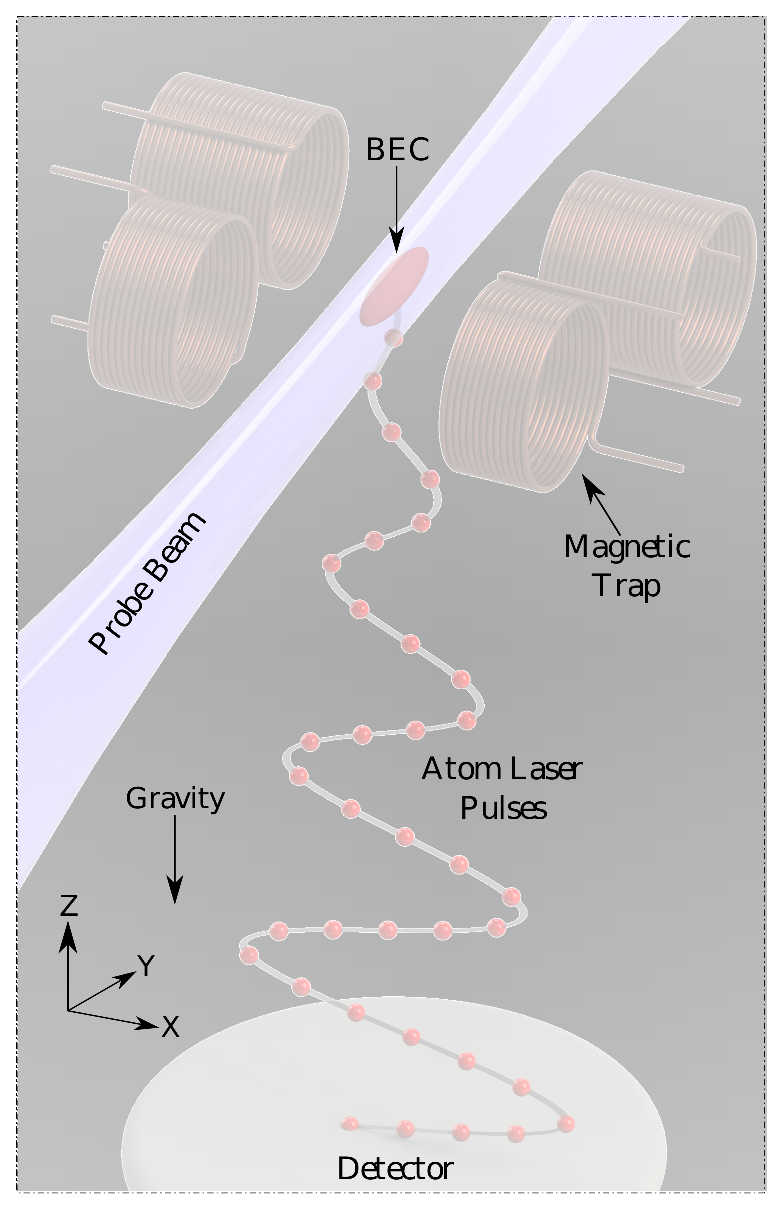
\includegraphics[width=8.6cm]{figs/exp_schematic}
\caption{
Schematic of the method}
\label{fig:schematic} 
\end{figure}

\section{Decisions}
\begin{outline}[enumerate]
    \1 Will refer to the effect on atoms as polarizability in the main text, 
        \2 will have a comment referring to soms where an explanation why Rayleigh Scattering is more appropriate
        \2 may need a change of title
    \1 Will refer to the tune-out by $\MetastableState\rightarrow\LowerStateManifold-\UpperStateManifold$
        \2 denotes the primary transitions that dominate the location of the tune-out
    \1 tune-out has a dash in it
    \1 will refer to frequency not wavelength
    \1 say test of QED not test of atomic structure
        \2 this points at the more fundmental nature of the work
\end{outline}{}

\section{Questions}
\begin{outline}[enumerate]
    \1 should we lead with Helium nuclear charge radius discrepancy or hydrogen proton size puzzle?
        \2 there is a bigger deal made about the hydrogen one
        \2 the discrepancy between \cite{Rengelink2018} and \cite{PhysRevLett.119.263002} is 1.8 sd
\end{outline}{}

\section{outline}
Main text should be about 2.5 pages long, 2500 words  including figures. Text must be understandable by gen scientist (non optical, cold atoms).
\begin{outline}[enumerate]
\1 Motivation
    \2 atoms are how we test physics
    \2 QED is very good
        \3 an example of its sucess
    \2 new challenges in the form of proton size 
        \3 muon hydrogen 
            %\4review by vassen https://science.sciencemag.org/content/358/6359/39
            %\3 review of the theory and experiment issues to resolve things https://www.epj-conferences.org/articles/epjconf/abs/2017/06/epjconf_conf2017_01023/epjconf_conf2017_01023.html
            \4 original muonic hydrogen \cite{Pohl2010} measurement (disagrees with prev electronic stuff)
            \4 muonic deterium \cite{Pohl669} (agrees with prev muonic hydrogen)
            \4 better normal hydrogen spectroscopy \cite{Bezginov1007}  now agrees with muon results
        \3 Helium \(\MetastableState \rightarrow \LowerStateManifold\)  spectroscopy 
            \4 \cite{PhysRevLett.74.3553} Shiner 1995, he3 charge radius 1.9506(4) fm, square difference he3-he4 1.059 \(\text{fm}^2\)
            \4 \cite{PhysRevLett.108.143001} Cancio 2012, he3 1.975(4) fm, square difference he3-he4 1.074(3)~\(\text{fm}^2\)
            \4 \cite{PhysRevLett.119.263002}, Zheng 2017, square difference he3-he4 1.028(2)~\(\text{fm}^2\)
        \3 Helium \(\MetastableState \rightarrow \SingletState \)spectroscopy
            \4 first \cite{vanRooij196} then improved \cite{Rengelink2018}, Rengelink 2018,  square difference he3-he4 1.041(7)~\(\text{fm}^2\) 
        \3 could be new physics relating to the proton structure, lepton interactions or QED itself.
    \2  using transition strengths is a novel way to investigate QED
        \3 eigenstate energy vs transtion strengths
        \3 other than hand waving is there anything concrete to suggest we can see problems not seen elsewhere? eg sensitivity to higher order terms ect.
\1 What is a tune-out
    \2 invisibility to atoms
        \3 like a jet plane
    \2 balance of transitions 
        \3 the weight is set by the distance to each transition and the transition strength
    \2 as a null measurement it provides a precision test
        \3 intensity calibration is not required, which limits other transition strength measurements
\1 why use this tune-out
    \2 Tune outs are as numerous as transitions
    \2 many tune-outs have been measured
    \2 This tune-out is better than other tune-outs
        \3 high sensitivity to QED
        \3 Helium means can do ab initio
            \4 Helium is a testbed (metastable lifetime, transition rates, isotope shifts, vims forbidden transition)
        \3 as a test of QED this is more/less sensitive to the nuclear size than the `proton size' measurements
\1 what we did
    \2 we measure the tune-out to be
        \3 value, unc
        \3 compare to theory
    \2 demanding from a theory point of view
        \3 what advances have been made?
    \2 exp advances that have been made
        \3 this tune-out is the weakest (weakest polarizability gradient) that has been measured
        \3 the reasons that make it sensitive also make it weak
        \3 Requires new methods for measuring the small potentials generated
        \3 sensitivity \& linearity   
\1 tune-out Method
    \2 How a tune-out is measured
        \3 polarizability creates an optical dipole potential 
        \3 measure potential as a function of frequency about tune-out
        \3 mention other methods
    \2 trap freq for tune-out
        \3 probe beam has a trap freq ( omega square is prop to polarizability)
        \3 combining two potentials gives a change in the net trap freq (sum of squares)
    \2 how we measure the osc freq
        \3 explained in detail elsewhere
        \3 give no mention of the aliasing in the main text
        \3 repeated out coupling of a small fraction of the atoms
        \3 some statement of how good this is 
            \3 trap freq measurement (15mhz,425Hz,30ppm)
            \3 specify the stability of the trap in multiple shots
        \3 corresponding potential depth sensitivity
\1 polarization dependence
    \2 tensor vector terms mean that tune-out is polarization dependent
    \2 want to compare with theory, however it is difficult to know the atomic polarization with sufficient accuracy
    \2 use TOSMHT which allows experimental extrapolation
    \2 measure tune-out as a function of polarization parameters
    \2 
\1 systematics
    \2 largest systematic shifts
    \2 should we have a table figure?
\1 implications
    \2 agreement with theory
\1 soms
    \2 link together Rayleigh scattering and polarizability
    \2 full protocol
        \3 use bec
            \4 decreases damping
        \3 biquick trap
        \3 on off measurement
        \3 probe beam is frequency and power stabilized 
        \3 cycle time, sensitivity scaling per run
    
    
\end{outline}

\clearpage

\section{Motivation}
%scraps
%The immense predictive power of theoretical atomic physics is a feat that is unrivaled elsewhere giving with agreement between experiment and ab-inito calculation reaching into the 15th decimal place \brycecom{cite}. %\brycecom{maybe first principles instead}
%However all is not harmonious, work in recent years has presented a discord, at the xx sigma level, between the proton radius measured using spectroscopy of the muonic versions of hydrogen/deuterium and more traditional approaches.
%Since the earliest days of spectroscopy, atomic physics has been fundamental to developing our understanding of the natural world.
By presenting a precisely measurable `test bed' atomic physics continually challenges the the fundamental theories that describe the interactions of charged particles. As a result quantum electrodynamics (QED) is unrivaled in its ability to make ab-inito predictions in a range of physical systemes.  However all is not harmonious, the `proton size puzzle' has presented discord, at the xx sigma level in its determination of the proton radius using spectroscopy of muonic hydrogen and deuterium compared to conventional approaches \cite{Pohl2010,Pohl669,Bezginov1007}. 
This trend is seen again in Helium where 
measurement of the \(\MetastableState \rightarrow \LowerStateManifold\) 
\cite{PhysRevLett.74.3553,PhysRevLett.108.143001,PhysRevLett.119.263002} and
\(\MetastableState \rightarrow \SingletState \) \cite{vanRooij196,Rengelink2018} transition frequencies yielding a discrepancies beyond four\brycecom{check} standard deviations in the derived Helium nuclear charge radius.

It is an open question where the answer to these challenges will lie with many proposals made such as new lepton sector physics \brycecom{cite} modifying the \(p-\mu\) interaction, nucleon structure physics \brycecom{cite}, subtle flaws in experimental methodology, or a limitation of QED itself.

BY determining the energy differences between atomic eigenstates these previous works all follow the well worn path towards tests of QED in atomic systems. Here we adopt a different approach that uses the precise ratio of transition strengths\(\bra{a}D\ket{b}\) between many states to provides an independent challenge to theoretical calculations in the hope of iluminating this problem further. Indeed this approach has \brycerev{greater/less} sensitivity to these nuclear sector effects and thus is a unique tool in seperating these effects.

\section{The tune-out}
\subsection{What is a tune-out measurement?}
An atom illuminated by a laser can be made invisible to the light by precisely tuning the laser to a frequency at which the atomic dynamic polarizability vanishes \cite{Drake2019}.
This ‘tune-out’ (TO) frequency \cite{PhysRevA.75.053612} occurs between transitions at the point where the sum of contributions to the dynamic polarizability for transitions below that frequency are balanced by those above it.In this balance the weight of each transition is set by the transition strength along with the difference between the laser and transition frequency.
%\brycecom{strictly speaking it doesn't have to be a laser...}\\
% \brycerev{removed `for a travelling light wave'}
In effect the atom becomes transparent to the light, and vice-versa, recalling the `stealth' invisibility of aircraft at (much lower) radar frequencies. 

The key innovation of the TO is that as a null measurement it does not require careful calibration of the light intensity that severely limits the precision of other transition strength measurement approaches.\brycecom{reference TO papers}


\subsection{Why use this one?}
As a feature of atomic systems TO's are as plentiful as transitions themselves however as a test of QED the TO of the \(\MetastableState\) (`metastable’) state of Helium (He*) between the \(\UpperStateManifold\) and \(\LowerStateManifold\) manifolds is uniquely suited.
The simplicity of Helium as an (approximately) 3 body system has a proven track record \brycecom{references: metastable lifetime, isotope shifts, transitions} of producing comparison with theoretical predictions with precision that are not currently possible in more complex species.
Over recent years precise calculations of this TO have shown that it is particularly sensitive to quantum electrodynamic (QED) contributions \cite{PhysRevA.88.052515} including finite nuclear size \cite{PhysRevA.99.040502} and retardation (finite wavelength) corrections \cite{Drake2019}.

\brycecom{should include other TO's around here somewhere without bashing them too much}
%Many tune-outs have been measured in a variitey of species Rb, Cs,... \brycecom{references}.
\kencom{I think we’ll need an analysis from Drake and Tang here of the relative magnitude of the QED
contributions, and their sensitivity to higher-order terms being omitted, in order to provide a
gauge of the meaningfulness of comparison with experiment.}


\section{What we did}
\subsection{Value}
Here we report a new measurement of this TO's frequency with a 20-fold improvement in the accuracy of the only previous measurement \cite{PhysRevLett.115.043004} producing the most precise measurement of transition rate information made to date. %\cite{2017arXiv170808200H} 
\brycecom{Q to Tang/Drake is this the best made over any species?}
This new experimental determination of xxx(x stat. ,  syst. xx )~MHz is xx standard deviations from the most recent theoretical value of xxx.xxx xxx (xx) MHz \cite{PhysRevA.99.040502}. 
\subsection{Theory advances}
\brycecom{will we be presenting new theory results in this work? If so some mention of the advances that have been made.}\\
\brycecom{Theory, Teaser of implications (1,2 sentences).}\\

The resulting measurement accuracy is at a level sensitive to QED contributions, and will further drive experiment and theory to determine whether the discrepancy reported here is due to previously undetermined theoretical contributions. Giving a window of insight into other outstanding disagreements.

\subsection{Exp Advances}

Intrinsically linked to the properties that give this TO its sensitivity to QED effects are those that produce its exceptional weakness, quantified by the gradient of the atomic dynamic polarizability with frequency about the TO. We therefore combine improvements in laser laser power with a novel method for the linear sensing of ultra weak potentials \(xx\cdot10^{\text{-}34}\text{~J}\cdot\text{s}^{\text{-}1/2}\), achieved through precise frequency measurement of the oscillatory motion of atoms in a confining potential. 

\section{Measurement Method}

\subsection{How do you measure a tune-out?}
Any measurement of a TO must somehow measure the interaction potential generated by a light field infringing on atoms as a function of frequency and extrapolate to the frequency that this interaction vanishes. To low orders \brycecom{in what?} this interaction potential is proportional to the dynamic atomic polarizability \(\alpha(\omega)\) and the light field intensity and is known as an optical dipole potential \brycecom{cite ODT for neutral atoms} however for accurate treatment at higher orders a Rayleigh scattering formalism must be employed (see soms)\cite{Drake2019}.
%this sentence is to contextualize the other methods used and unify them under one picture so that we can show how our method beats out all of them on the level playing field of potential
Previous work has developed a number of different approaches to measure the potential that is generated about the tune out such as atom interferometery and motional bloch oscillations in an optical lattice \brycecom{references}. 

\subsection{Trap freq for TO}
The approach taken here measures the spatial oscillation frequency of atoms that are exposed to a focused probe beam overlapped with a stable, harmonically confining, magnetic trap. The resulting combination is given by,  \(\Omega_{\text{net}}^2=\Omega_{\text{trap}}^2+\Omega_{\text{probe}}^2\) where \(\Omega_{\text{net}}\), \(\Omega_{\text{trap}}\), \(\Omega_{\text{probe}}\) denote the trap frequency of the combined, probe and trapping potentials respectively. As the probe beam frequency scales as \(\Omega_{probe}^2\propto \alpha(\omega) P\), where P is the power of the beam,the combination of power stabilization of the probe beam and a calibration procedure to determine \(\Omega_{\text{trap}}\) produce a sensitive determination of a signal linearly proportional to \(\alpha(\omega)\).

%\(\Omega_{\text{probe}}^2=\Omega_{\text{net}}^2-\Omega_{\text{trap}}^2\)

\brycecom{is \(\Omega_{\text{C}}\) for combined or \(\Omega_{\text{N}}\) for net better?}
\subsection{trap freq measurement}
We have developed a precision trap frequency metrology approach detailed elesewhere \brycecom{Ref trap freq paper}. In brief the method uses repeated sampling of the momentum of atoms oscillating in a confining harmonic trap. Fitting the measured momentum as a function of time with a dampened sine wave model allows for the determination of the trap frequency to a precision of 30~ppm in a single experimental realization. Momentum sampling is realized by transferring a small fraction of atoms confined in a magnetic trap from the magnetically repulsive ($m_J=1)$) state to the insensitive ($m_J=0$) state with a short radio frequency pulse (atom-laser) allowing the mean momentum to be measured with a detector located below the trap. 
To reduce the damping that ultimately limits the interrogation time the starting sample of atoms used is cooled to degeneracy to form a Bose-Einstein condensate (BEC). The oscillating motion is then induced in a single axis with a brief displacement of the trap center. 

In a measurement of the TO the net trap frequency is measured as a function of the probe beam (optical) frequency with frequent calibrations of the confining potential trap frequency in order to eliminate any long term drift. Each measurement starts with a new sample of He* which are depleted over the course of the trap frequency measurement (2~s) . 
The small scan range of \(\omega\) used in our experiment permit the simple linear extrapolation of (optical) frequency to the null of the polarizability signal giving the TO frequency \(\omega_{\text{TO}}\) ( \(\alpha(\omega_{\text{TO}})=0\) ).


\begin{figure}[H] 
\centering
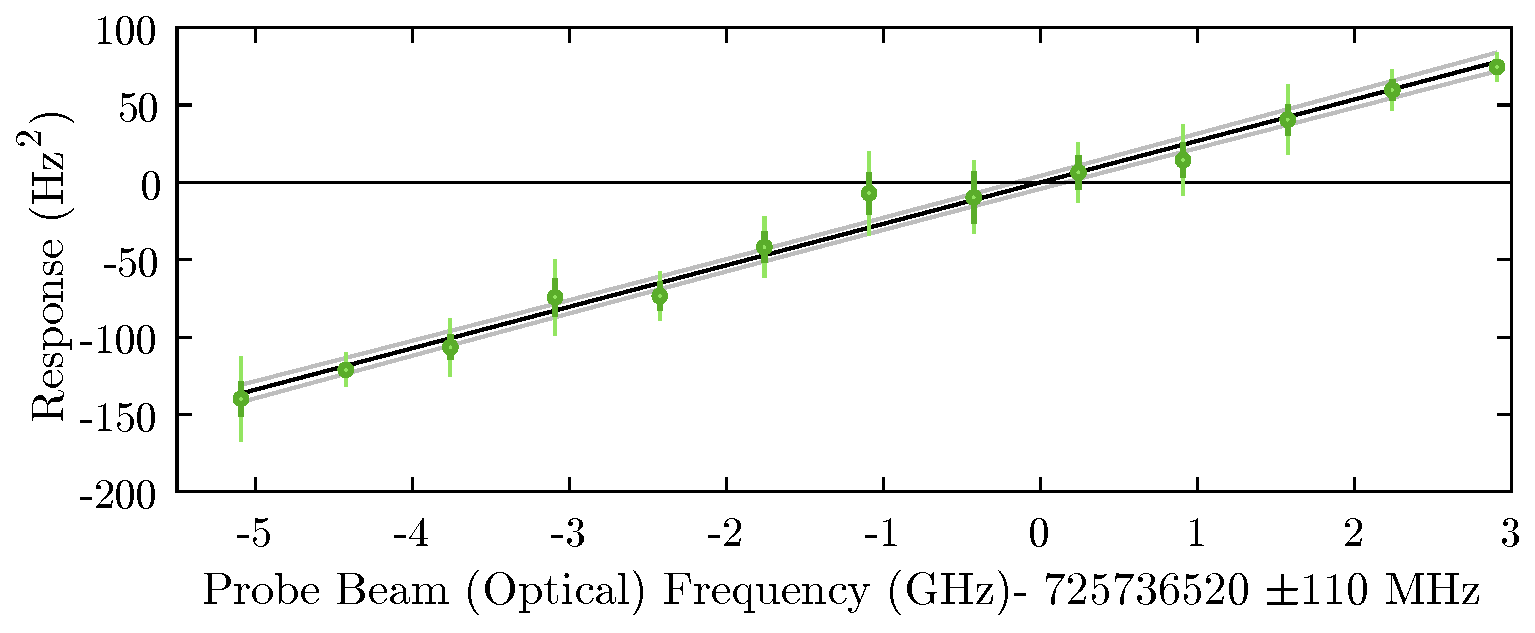
\includegraphics[width=8.6cm]{figs/signal_vs_opt_freq.eps}%[width=500px]
\caption{ 
Experimental measurement of the TO frequency.\brycecom{Find scan that is centred, }}
\label{fig:to_meas_sig_freq}
\end{figure}

\section{polarization dependence}

As the strength of each transition in an atom has an dependence on the polarization and relative orientation of the light field the dynamic atomic polarizability also caries this dependence. This complicates the comparison with theory as the tune out measurment must be made with a well known polarization state. The net polarizability is given by 
\begin{equation}
    \alpha(\omega) = \alpha^S(\omega) - 
    \frac{1}{2} \mathcal{V} \cos \left( \theta_k \right) \alpha^V(\omega) + 
    \frac{1}{2} \left(3 \sin^2\left( \theta_k \right) \left(\frac{1}{2} +  \frac{R(\mathcal{Q},\theta_{\text{rot}})}{2}\right) -1 \right) \alpha^T(\omega) 
    \label{eq:polarizability_full}
\end{equation}
where \(\mathcal{Q}, \mathcal{V}\) are the 2nd and 4th stokes parameters in the laboratory orientation, \(\theta_{\text{rot}}\) is the rotation angle between the laboratory polarization and the atomic polarization, \( R(,\theta_{\text{rot}}) \) is the rotation transform, \(\alpha^S(\omega),\alpha^V(\omega),\alpha^T(\omega)\) are the frequency dependent scalar vector and tensor components of the polarizability and \( \theta_k\) is the angle between the probe beam and the magnetic field. 
To compare with theory we measure the TO's dependence on the probe beam polarization and extrapolate to the polatization state \( \mathcal{Q}=-1, \mathcal{V} =0 \) giving . 
\begin{equation}
    \alpha(\omega) = \alpha^S(\omega) - \frac{1}{2} \alpha^T(\omega) 
    \label{eq:polarizability_full}
\end{equation}
By finding the tune-out of the scalar minus half the tensor polarizability (TOSMHT) the measurement is insensitive to the angles ( \(\theta_{\text{rot}}, \theta_k \) ) which would otherwise limit the precision of the measurement.
The protocol for this measurement is illustrated by considering a perfectly linearly polarized probe beam which used to make a number of TO measurements as a function of the polarization angle. This then traces out a sinusoidal dependence with one of the extrema equal to the TOSMHT. %To determine which we require either another measurement with a different \( \theta_k\) or the sign of the tensor component of the polarizability from theoretical calculations. 
To determine which use sign of the tensor component of the polarizability from theoretical calculations which is well determined with a small QED contribution. 
To tolerate the imperfections of the light polarization that give a circular component of the probe we employ a more sophisticated fitting scheme that inculudes the dependence on \( \mathcal{V} \).

\section{systematics}
A dominant systematic effect in our measurement is the determination of the light polarization. The probe beam passes through multiple optics and a vacuum window before it interacts with the atoms. To constrain the error in the polarization measurement made outside the vacuum chamber we measure the polarization once the beam has exited the vacuum system, we find agreement in the derived TOSMHT values to within 40~MHz.

In contrast to absorption spectroscopy where the sensitivity to light at some detuning from the resonance falls off quickly, the TO measurement has a sensitivity that increases super-linearly with detuning. This then requires careful filtering and characterization of the background light to prevent a large shift from a small amount of light with a large detuning. A multi 4 stage filtering system is employed and an investigation into the shift performed by removing these filters produced results that are consistent with no effect and an uncertainty of 30~MHz.

The linearity of the measurement is required for the linear extrapolation used to be valid. This is quantified to give a xx~MHz shift with an uncertainty of xx~MHz

\section{implications}












\begin{acknowledgments}
This work was supported through Australian Research
Council (ARC) Discovery Project Grant No. DP160102337. 
D.K.S. is supported by an Australian Government Research Training Program (RTP) Scholarship.
S. S. H. is supported by ARC Discovery Early Career Researcher Award No. DE150100315.
\end{acknowledgments}

\bibliographystyle{apsrev4-1}
\bibliography{to_v2}

\clearpage
\section*{{\large{Supplementary Materials}}}\label{section:SOMs}

\subsection{full protocol}

The experiment begins with the production of a $^{4\!}\text{He*}$ BEC through multiple laser and evaporate cooling stages \brycecom{cite prev work}. \brycecom{should we spcify isotope?}\\
These atoms are confined in a stable, harmonicaly confining, magnetic trap \brycecom{cite biquic} with trap frequencies \(\left( \omega_x,\omega_y,\omega_z \right) \approx 2\pi \left(5x,4xx,4xx \right)\textrm{Hz}\). A power and frequency stabilized probe beam with its focus overlapped on the magnetic trap minimum is then gradualy turned on, producing a small shift in the net trap frequency.
To induce a center of mass motion, predominantly in the xx axis, a short (xx~{\textmu}s) pulse of current is applied to a coil near the trap. 
The resultant momentum of these oscillating atoms is then repeatedly sampled over a period of xx seconds. 
The determined mean momentum of each sample is used to fit of a dampened sine wave model extracting the net trap frequency. 
Every alternate experiment the probe beam is not applied, measuring the magnetic trap frequency in isolation, and in turn the probe beam trap frequency as \(\Omega_{\text{probe}}^2=\Omega_{\text{net}}^2-\Omega_{\text{trap}}^2\). The TO for a particluar polarization state ($\omega_{TO}(\mathcal{V},\mathcal{Q})$) is measured by repeating these experiments as the probe beam optical frequency is changed, extrapolating to the optical frequency where the probe beam trap frequency is zero.\\
\brycecom{I think somewhere it should be explained that polz. is approx. linear about TO, and that \(\omega_{\text{probe}}^2\) is linear with polz.}\\
\brycecom{Can we leave out the probe beam freq stabilization through the wavemeter from this section?}\\ 


\subsection{Scraps}

(refering to theory calcs) Such calculation have shown that retardation (finite frequency) corrections are also important, as shown when the TO frequency calculation is formulated as a zero in the Rayleigh scattering cross-section for an atom interacting with a plane electromagnetic wave \cite{Drake2019}.

A TO frequency is a frequency of light at which the dynamic dipole polarizability of some state is zero.
Originally proposed as a way to independently manipulate multiple atomic species \cite{PhysRevA.75.053612}, its function as a null measurement of polarizability makes it well suited as a high precision test of atomic structure theory  \cite{PhysRevA.88.052515}.
%(that does not depend on accurate knowledge of the light field intensity)
The 413nm TO frequency for the $2\,^{3}S_{1}$ state of Helium is unique in that it is particularly sensitive to the QED effects that are the focus of our study. In particular, Mitroy and Tang have shown \cite{PhysRevA.88.052515} that a determination of this TO frequency to an uncertainty of 100~fm (175~MHz) would set a new record for the most precise measurement of transition rate information made in a atomic system. 
Following the first measurement to 4~GHz (2~pm) by the ANU group \cite{2017arXiv170808200H,PhysRevLett.115.043004}, surpassing then-current theoretical predictions, a theoretical campaign has improved the prediction of the TO frequency to the level of 70~MHz (40~fm) \cite{PhysRevA.93.052516,manalothesis,Drake2019,PhysRevA.99.040502}, urging an improved measurement campaign.


%{\em Experimental setup.---}
 The atom laser beam in our experiments is produced by illuminating a magnetically trapped BEC of metastable Helium (He*) atoms, in the long lived $2^3S_1$ state \cite{Hodgman2009a}, with a  pulse  of radio frequency (RF) radiation.
 The RF pulse, resonant with the Zeeman splitting between the $m_J{=}+1$ (trapped) and $m_J{=}0$ (untrapped) internal states at ${\sim} 700$~kHz, transfers atoms from the cigar-shaped trap, ${\omega_r,\omega_z}\approx2\pi\times{550, 50}$~Hz, into the atom laser beam. 
 The short pulse duration (${\sim}10$~\textmu{}s) leads to a large broadening in the frequency spectrum, resulting in a nearly uniform outcoupling into the atom laser beam despite the inhomogeneous magnetic field of the trap.
 Atoms then expand under the (cigar-shaped) repulsive mean field potential of the trapped condensate to form a thin disk with a (far field) spatial ratio of approximately ten to one. The subsequent passage of the trapped BEC through the atom laser can thus be treated as a 2D problem.

 The atom laser then falls under gravity a distance of ${\sim} 850$~mm (time of flight ${\sim} 416$~ms) where the atoms are imaged in the far-field with full three dimensional resolution using an $80$~mm diameter multi-channel plate and delay line detector (DLD) \cite{Manning:10}. 
 The large internal energy of the $2^3S_1$ state of He* (${\sim} 20$~eV) allows the DLD to reconstruct individual atoms at a spatial resolution of ${\sim} 120$~\textmu{}m, a temporal resolution of ${\sim} 3$~\textmu{}s \citep{SOMs} and a quantum efficiency of ${\sim} 10\%$.
 \footnote{Measured using the normalized variance of a scattering halo as in \cite{PhysRevLett.108.260401}.}

To improve on previous work we combine a substantial increase in laser power with an improved optical potential measurement technique based on precision trap frequency metrology. Using the unique detection ability available to He* we repeatedly sample the momentum of an oscillating Bose Einstein Condensate in a magnetic trap with a weak, pulsed, atom laser. The trap frequency can then be determined in a single experimental realization with an accuracy exceeding previous approaches by orders of magnitude.
We apply a probe beam near the TO frequency to perturb the trap frequency.
By then measuring the dependence of the trap frequency on the applied probe beam frequency we produce a sensitive measurement of potential and in turn the TO frequency. We discuss extensions of this method beyond mean-field induced bandwidth limits by a reconstructive aliasing technique.

\subsection{Method}
The TO analysis consists of two broad stages: in the first the frequency(wavelength) of light at which no perturbation of the atoms is observed is determined for some input polarization state. Then many of these measurement's (with varying degrees of circularity and linear orientation) are combined and fit in stokes space for the TO Scalar Minus Half Tensor (TOSMHT) which may be compared with theory.
The analysis for a given polarization generally consists of 100's of shots(BEC's) grouped together into a run which is converted to a measured TO for that polarization.




\subsubsection{Method Part 1: Measuring the TO for a given polarization}
At its core this involves measuring the trap frequency as a function of the applied probe beam frequency(wavelength). 

For each experimental realization we create a new BEC through a combination of laser cooling and evaporative techniques in a magnetic trap. The magnetic trap is a bi-planar quadrupole Ioffe trap \cite{Dall2007a} with trapping frequencies of 425,420,50 Hz[todo verify y,z].
The probe beam which is overlapped on the BEC with a waist of (xxum) and aligninged along the weak axis of the trap is then either turned on in the case of a probe measurement or kept blocked for a calibration measurement. In the case of a probe measurement the net trap frequency will then be altered in proportion to the polarizability and second derivative of the intensity.

To measure this change in trap frequency A brief ($xxus$) pulse of current is applied through a small coil near the BEC is used to induce oscillation predominantly in the x direction. The oscillating BEC is partially out-coupled with short ($\sim\text{xx}\mu s$) pulses of RF radiation resonant with the ($\sim 1.7MHz$) $m_J=+1,0$ state splitting at the center of the trap, these pulses are repeated every (xx ms). The atoms that are transferred to the $m_J=0$ state are unaffected by gravity and fall 852~mm to a multi-channel plate and delay line detector \cite{Manning:10}. The large internal energy of the atoms ($\sim 20$~eV) allows detection with a spatial (temporal) resolution of  $\sim 120$~\textmu{}m ($\sim 3$~\textmu{}s) \cite{PhysRevA.97.063601} and a detection quantum efficiency of ${\sim} 10~\%$.  

The mean position (and time) of each atom laser pulse is used to infer the in trap momentum before out coupling. By fitting xx of these measurements with an exponentially dampened sine wave we are able to precisely determine the trap frequency with a single experimental realization.

To partially compensate for the decreasing atom number, which would otherwise proceed as a geometric series and greatly increasing the velocity variation of later pulses, the RF power is increased as the pulse number increased.

By repeating the above experimental procedure with the probe beam on and blocked we can accurately determine the change in trap frequency from the applied probe beam. 

While in principle this fitting procedure could be done for all 3 axes the long Raleigh length of the probe beam and weak trap frequency in that axis  induces only a small change in trap frequency in the weak axis of our trap.  inducing oscillations in all axes can produce complex cross coupling effects and so we chose to induce the oscillation predominately in the X (tight horizontal) axis of our trap.


A is then fit to these positions in each dimension to extract a measurement of the net trap frequency in each axis. 
In total the model has the damping term, fundamental frequency,phase and amplitude
  
Then the shots are split depending on if they are calibration or not.  
The calibration shots are then used to create a interpolated calibration model (for each of the fit parameters) in order to remove long term drifts in the trap freq.
the signal for the non calibration shots is taken as the square difference in the fit frequency to this calibration model.
the signal is combined with the measured average optical frequency during the probe beam interrogation.
The signals are grouped into scans of optical frequency across the TO and fit with a linear model to estimate the TO for that scan.
A measurement of the TO for a given polarization consists of ~5 of these scans.

\begin{figure}
\centering
\includegraphics[width=\textwidth]{figs/method_stage1_processing_schematic}
\caption{
Schematic of the method to determine the TO for a given polarization state. (left) The mean position of each pulse of the atom laser in the x axis is determined and converted to effective velocity Many experimental realizations combined for this histogram).  (Top) The velocity as a function of time is then fit with a dampened sine wave model (single experiential realization shown) to determine the trap frequency. (Bottom) The difference in the square trap frequency between runs with the probe beam on and off is used as the response proportional to the polarizability. A linear model is fit to this response as a function of probe beam (optical) frequency (data is shown for 100's of shots) and the x intercept is determined as the measurment of the TO frequency for this polarization state.}
\label{fig:stage_1_processing_schematic} 
\end{figure}

\subsubsection{Method Part 2: Measuring the TOSMHT}
While perfomed with record potential sensitivity the results from part 1 cannot be compared to theory as they require the precise measurement of the light polarization state along with the B-feild and probe beam pointing, experimentally these last two parameters are difficult to determine with reasonable precision. We instead adopt a different procedure in which we extrapolate to the linear polarization state with the rotation that gives the largest tune-out (optical) frequency corresponding to when $\theta_p=\pi/2$. This case corresponds to the scalar polarizability minus half the tensor polarizability (TOSMHT)
\begin{equation}
    \alpha(\omega) = \alpha^S(\omega) - \frac{1}{2}  \alpha^T(\omega) .
\end{equation}
In this way only a single parameter is required from theory, namely the sign of the tensor polarizability around the TO wavelength. This approach assumes that the tensor and vector polarization is approximately constant about the TO.

Experimentally this procedure is done by performing a fit of the expression derived later to the measured TO values frequencies, and polarization measurements at a range of $\lambda/2$, $\lambda/4$ wave-plate angles.
\begin{equation}
    \omega_{TO} = \omega^{S}_{TO} + \frac{1}{2} \beta^V \cos \left( \theta_k \right) \mathcal{V}  - \frac{1}{2} \beta^T \left(3 \sin^2\left( \theta_k \right) \left(\frac{1}{2} +  \frac{\mathcal{Q}(\theta_{rot})}{2}\right) -1 \right)
\end{equation}
The fit terms are $\omega^{S}_{TO}$, $\theta_{rot}$, $\beta^V$, $\beta^T$. The last three terms are interdependent however the extrapolation to the state Q=-1 gives the desired TOSMHT.
Where the term $\mathcal{Q}(\theta_{rot})$ is given by.
\begin{equation}
 \mathcal{Q} =\frac{p_{max}-p_{min}}{p_{max}+p_{min}} \cos(2(\theta_{rot}+\theta_{P_{min}}))
\end{equation}
Where $p_{min}$,$p_{max}$ correspond to the minimum(maximum) light power measured through a polariser as it is rotated, $\theta_{P_{min}}$ is the angle in the lab frame of this minium power, $\theta_{rot}$ accounts for the measurement of polarization done in the lab frame that does not necessarily correspond to $\theta_\varepsilon$ and must be rotated into this frame.



The data for this fit consists of measured values of the polarization state ($p_{max}$,$p_{min}$,$\theta_{P_{min}}$) as the independent variables (which is altered with waveplate(s) angle(s)) and the measured TO for each scan as the dependent variable. The fit is weighted by the square of the uncertainty in each TO measurement $1/\sigma^2_{\omega_{TO}}$. The measured TO for each xx shot scan over wavelength for a given polarization is included in the fit as its own data point. The fit is conducted with a global least squares prefitter that is constrained such that $-\pi/4<\theta_k<\pi/4$ and  $\beta^T>0$ which is then fed to an unconstrained fitter. The statistical error in the determined TOSMHT is determined with a bootstrapping technique  \href{https://github.com/brycehenson/bootstrap_error}{bootstrap code}. 



For display the $\mathcal{Q}$ value in the atomic frame is calculated using the fit $\theta_{rot}$ and the measured TO is displayed as a function of $\mathcal{Q}$,$\mathcal{V}$. For display each polarization is combined, with the uncertainty weighted mean, and standard error of the weighted mean \href{https://github.com/spicydonkey/sewm}{sewm code} along with unweighted standard deviation calculated.




It is clear here that the estimated statistical error in the determined TO frequency for each scan is far less than spread between the the model and the data. (factor of 6 between SEWM of combined data and the sd of redisulas, will calc for each unbinned data pt) We attribute this to imperfections in the polarization measurement and variation of the magnetic field pointing.

\newcommand{\subfigwidth}{0.3\linewidth}

\begin{figure}
    \centering
    \subfigure[]{\includegraphics[width=\subfigwidth]{figs/3d_omega_vq_perspective1.png}}
    \subfigure[]{\includegraphics[width=\subfigwidth]{figs/3d_omega_vq_perspective2.png}}    
    \subfigure[]{\includegraphics[width=\subfigwidth]{figs/3d_omega_vq_perspective3.png}}  
    \subfigure[]{\includegraphics[width=\subfigwidth]{figs/3d_omega_vq_perspective4.png}}  
    \subfigure[]{\includegraphics[width=\subfigwidth]{figs/3d_omega_vq_perspective5.png}}  
\caption{ Fit to the measured TO $\omega_{TO}$ as a function of the  $\mathcal{Q}$,$\mathcal{V}$ polarization parameters. Black Square shows the extrapolated data point. }
\end{figure}

\begin{figure}[h!]
\centering
\includegraphics[width=8.6cm]{figs/q_dependence.eps}
\caption{ 
Dependence of the measured TO on $\mathcal{Q}$ when projected to  $\mathcal{V}=0$. The thin error bars show the standard deviation of the data that is used to make up the presented point, thick error bars show the estimated standard error in the weighted mean. \brycecom{use same symbol in graph as text}
}
\end{figure}

\begin{figure}[h!]
\centering
\includegraphics[width=8.6cm]{figs/v_dependence.eps}
\caption{Dependence of the measured TO on $\mathcal{V}$ when projected to  $\mathcal{Q}=-1$. The reader should not that some values on this plot are not physical (eg  $\mathcal{V}=1,\mathcal{Q}=-1$) however the relation is linear. \brycecom{TODO: project to $\mathcal{Q}=0$ instead to prevent confusion} \brycecom{use same symbol in graph as text}
}
\end{figure}



A substantial potential systematic error in our measurement is the error between the measured polarization state and what the atoms experience. The data presented above is produced using polarizaiton measurement's made once the beam exits the vacuum system. We estimate this polarization determination error by comparing this measurement with the the TOSMHT determined using the polarization measured before the vacuum system. 


\begin{table}[H]
\centering
\begin{tabular}{l|r|r|r}
\hline
Value                            & Freq (MHz)  & Unc(MHz) & Power (uw)  \\
\hline
Theory scalar                    & 725 738 782 & 70      &           \\
Theory SMHT                      &725 736 428 & 53      &           \\
\hline
\multicolumn{4}{l}{Experiment - 725 730 000}\\
\hline
post vac. polz. raw meas    &  725 736 812       & 33       &           \\
post vac. polz. fit         & ... 6 835       & 45       &           \\
\quad- theory SMHT                    &384      & 70      &           \\
pre vac. polz. cent         &... 6 614       & 53       & 107       \\
pre vac. polz. left         & ... 6 855       & 42       & 23        \\
pre vac. polz. right        & ... 7 157       & 51       & 15        \\
pre vac. power weight       & ... 6 709       & 40       &           \\
\quad- theory SMHT                    & 281      & 66      &           \\
pre vac. sqrt. power weight & ... 6 786       & 32       &           \\
\quad- theory SMHT                    & 358      & 62      &           \\
                                 &             &          &          
\end{tabular}
\caption{Scalar value from \cite{PhysRevA.93.052516}, correction to SMHT applied using the shift in ``Response to Bryce's questions'' of -0.980 pm.}
\end{table}

From this it seems that we do not agree with theory.




\subsection{Polarizability of Atoms in an Arbitrary light field}\label{sub_sec_to_polz_deriv}
This derivation follows a lot of \cite{LeKien2013} .
Consider the interaction between an atom (in an external magnetic field \textbf{B} and Zeeman sublevel \(\ket{JM}\)) and a monochromatic classical light field given 
\begin{align}
    \textbf{E} &= \frac{1}{2} \mathcal{E} \textbf{u} e^{-i \omega t} \, + \, \text{c.c.},
\end{align}
where \(\omega\) is the angular frequency, \(\mathcal{E}\) is the electric field amplitude, and \textbf{u} the complex polarization vector. Note that only the real component of \textbf{E} has a physical meaning. For a strong enough magentic field (specifically when the off-diagonal terms are much smaller than the   Zeeman splitting of the sublevel, see \cite{} for more detail) the dynamic polarizability of the atom is:
\begin{equation}
    \alpha(\omega) = \alpha^S(\omega) + C \alpha^V(\omega) \frac{M}{2J} + D \alpha^T(\omega) \frac{3M^2-J(J+1)}{2J(2J-1)}
    \label{eq:polarizability_full}
\end{equation}

where \(\alpha^S\), \(\alpha^V\), and \(\alpha^T\) are the conventional scalar, vector, and tensor polarizabilities respectively. If we assume that the B-field is pointing along the \textit{z}-axis then the Coefficents \(C\) and \(D\) are given by:
\begin{align}
    C &= 2 \text{Im}(u_x^* u_y),\\
    D &= 3|u_z|^2 -1
\end{align}
We can furthermore define these constants in terms of experimentally measurable variables (see ... for derivations)
\begin{align}
     C &= - \mathcal{V} \cos \left( \theta_k \right), \\
     D &= 3 \sin^2\left( \theta_k \right) \left(\frac{1}{2} +  \frac{\mathcal{Q}}{2}\right) -1 
\end{align}
where \(\mathcal{V}\) is the fourth stokes parameter, whose magnitude is given below and sign depends on the handedness of the light. \(\mathcal{Q}\) is the second stokes parameter in the preferred atomic rotation.

\begin{align}
     \mathcal{Q} &=\frac{p_{max}-p_{min}}{p_{max}+p_{min}} \cos(2\theta_\varepsilon), \\
     |\mathcal{V}| &= \frac{2\sqrt{p_{min}p_{max}}}{p_{min}+p_{max}},\\
     \cos(\theta_\epsilon) &=\text{Re}\left\{\textbf{u}\right\}\cdot(\textbf{B}\times \hat{k})
\end{align}


Near the TO the the full dynamic polarizability \(\alpha(\omega)\) along with the scalar component of the polarizability \(\alpha^S(\omega)\) can be approximated by their first order linear Taylor expansions about their respective zero points (\(\omega_{TO}\), \(\omega^{S}_{TO}\)):
\begin{align}
    \alpha(\omega) &= \alpha(\omega_{to}) + \derivn{\alpha(\omega)}{\omega}{{}}(\omega-\omega_{TO})=\derivn{\alph
    a(\omega)}{\omega}{{}}(\omega-\omega_{TO}), \\
    \alpha^S(\omega) &= \alpha^S(\omega^{S}_{TO}) + \derivn{\alpha^S(\omega)}{\omega}{{}}(\omega-\omega^{S}_{TO})= \derivn{\alpha^S(\omega)}{\omega}{{}}(\omega-\omega^{S}_{TO})
\end{align}
where \(\omega_{to}\) is the desired term. Note that for these approximations to be valid we need to only consider a small range about the respective zero values (\(\omega_{to}\), \(\omega^{S}_{TO}\)), and as a consequence of this we must assume that the difference between these values is small. Substituting we obtain:
\begin{align}
    \derivn{\alpha(\omega)}{\omega}{{}}(\omega-\omega_{TO}) &= \derivn{\alpha^S(\omega)}{\omega}{{}}(\omega-\omega^{S}_{TO}) + C \alpha^V(\omega) \frac{M}{2J} + D \alpha^T(\omega) \frac{3M^2-J(J+1)}{2J(2J-1)}
\end{align}
The major contribution to the rate of change of the dynamic polarizability (\(\derivn{\alpha(\omega)}{\omega}{{}}\)) is from the scalar polarizability (or equivalently that the vector and tensor terms are approximately constant over the range being considered), hence \(\derivn{\alpha(\omega)}{\omega}{{}} \simeq \derivn{\alpha^S(\omega)}{\omega}{{}}\). Rearranging and making this approximation into equation \ref{eq:polarizability_full} we obtain:
\begin{align}
     \omega-\omega_{TO} &= \omega-\omega^{S}_{TO} + C \beta^V(\omega) \frac{M}{2J} + D \beta^T(\omega) \frac{3M^2-J(J+1)}{2J(2J-1)}\\
    \omega_{to} &= \omega^{S}_{TO} - C \beta^V \frac{M}{2J} - D \beta^T \frac{3M^2-J(J+1)}{2J(2J-1)},
\end{align}
where $\beta^{(V,T)} = \alpha^{(V,T)}(\omega_{TO}) /\derivn{\alpha(\omega)}{\omega}{{}}$ are the reduced vector and and tensor contributions, $\omega^{S}_{TO}$ is the scalar TO frequency. We are interested in the $2^3S_1$ state $\ket{J=1,M=1}$
\begin{align}
    \omega_{TO} &= \omega^{S}_{TO} - C \beta^V \frac{1}{2} - D \beta^T \frac{1}{2},\\
    \omega_{TO} &= \omega^{S}_{TO} + \frac{1}{2} \beta^V \cos \left( \theta_k \right) \mathcal{V}  - \frac{1}{2} \beta^T \left(3 \sin^2\left( \theta_k \right) \left(\frac{1}{2} +  \frac{\mathcal{Q}}{2}\right) -1 \right)
\end{align}
If we set \(\mathcal{V}=0\) and \(\mathcal{Q}=-1\) we obtain \(\omega_{TO} = \omega^{S}_{TO} + \frac{1}{2} \beta^T\) which is the TO frequency for the dynamic polarizability \(\alpha(\omega) = \alpha^S(\omega) - \frac{1}{2}  \alpha^T(\omega)\).




\subsection{Systematics}

%\section{Systematics}
%Bryce TODO
% - estimate background light power (and include measurements of attenuation)

% we use the dependence on the spectral filtering in order to estimate the error in the measured TO \cite{PhysRevA.92.052501}
% \begin{outline}
% \1 \cite{PhysRevA.92.052501} used depenednce on width of filtering
% \end{outline}

\begin{table}[h]
\centering
\begin{tabular}{l|r|r|r}
\hline
Term              & Estimate & Statistical Uncertainty & Systematic Uncertianty \\
\hline
Measured Value      & 725735154             & 50    & 150            \\
Broadband Light     & ?                     & ?     & ?        \\
Method Linearity    & ?                     & ?     & ?             \\
Wave-meter          & 0                     & $<1$    & 4             \\
\hline
\multicolumn{4}{l}{Theory}\\
\hline
Hyp. Polz           & ?                     & ?     & ?        \\
Magnetic field      & ?                     & ?     & ?             \\
DC Stark Shift      & ?                     & ?     & ?             \\
Thermal Hyperpolarizability Shift & ?     & ?     & ?            \\
Mean Field          & ?                     & ?     & ?             \\
\hline
Total               &  ?                    &  ?    & ?
\end{tabular}
\caption{Measured TO frequency, all values are in MHz}
\label{tab:5/tc}
\end{table}



\subsubsection{Hyperpolarizability}

\begin{figure}[h!]
\centering
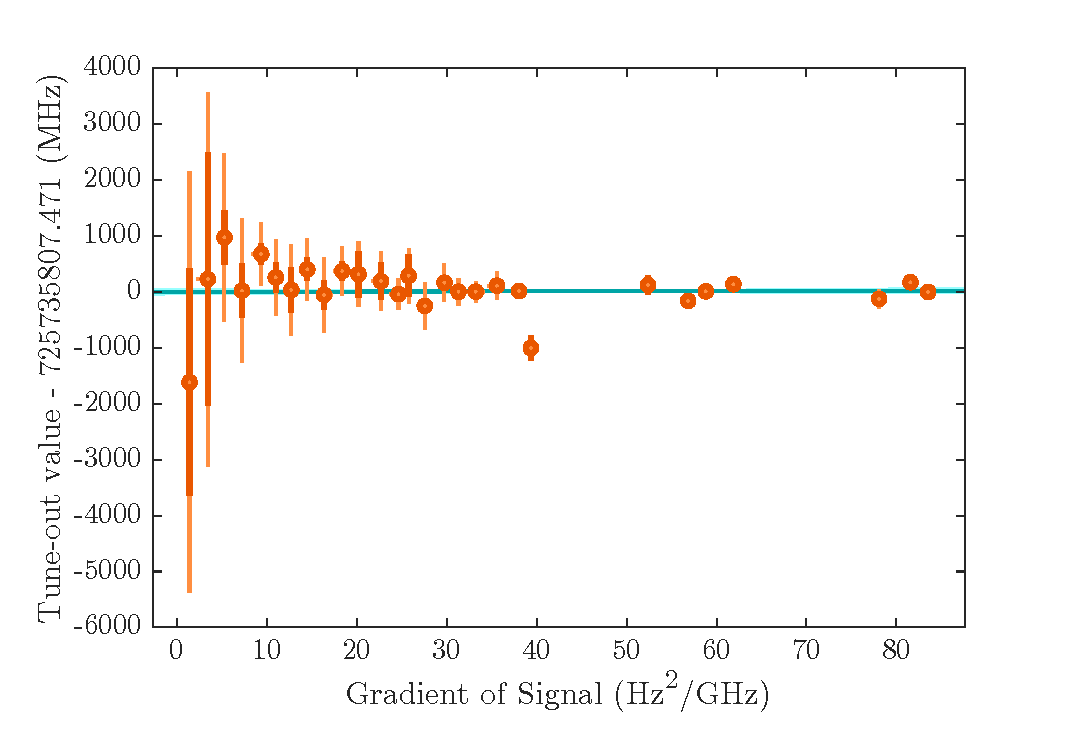
\includegraphics[width=8.6cm]{figs/grad_dep.eps}
\caption{ Dependence of the measured TO value on light field intensity. The signal gradient is used as a proxy of the light field intensity that is less sensitive to alignment drifts. $y=(725735807.471301\pm55)+(0.226\pm1.15)x$ Horizontal bars show range that is averaged over.
}
\end{figure}

\subsubsection{Method Linearity}

\begin{figure}[h!] 
\centering
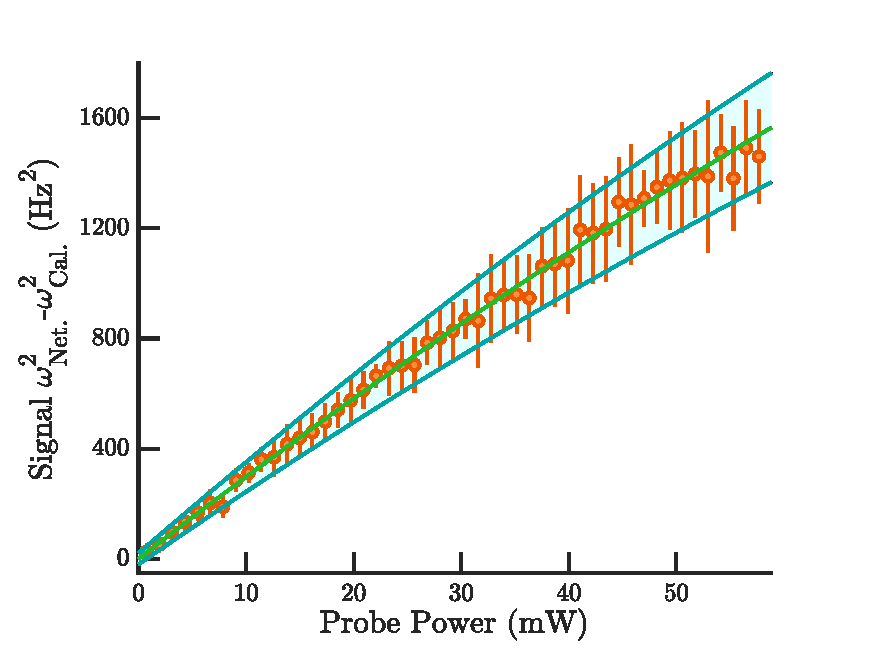
\includegraphics[width=8.6cm]{figs/linearity.eps}
\caption{ 
linearity of the method with the probe beam set 20GHz above the TO $y=30.3\cdot x-0.06\cdot x^2$. Terms are added until they are not statistically significant, the y intercept is within error of zero. The shaded region shows the observation one standard deviation. }
\label{fig:to_lineaity}
\end{figure}

\subsubsection{Background light}

\begin{figure}[h!]
\centering
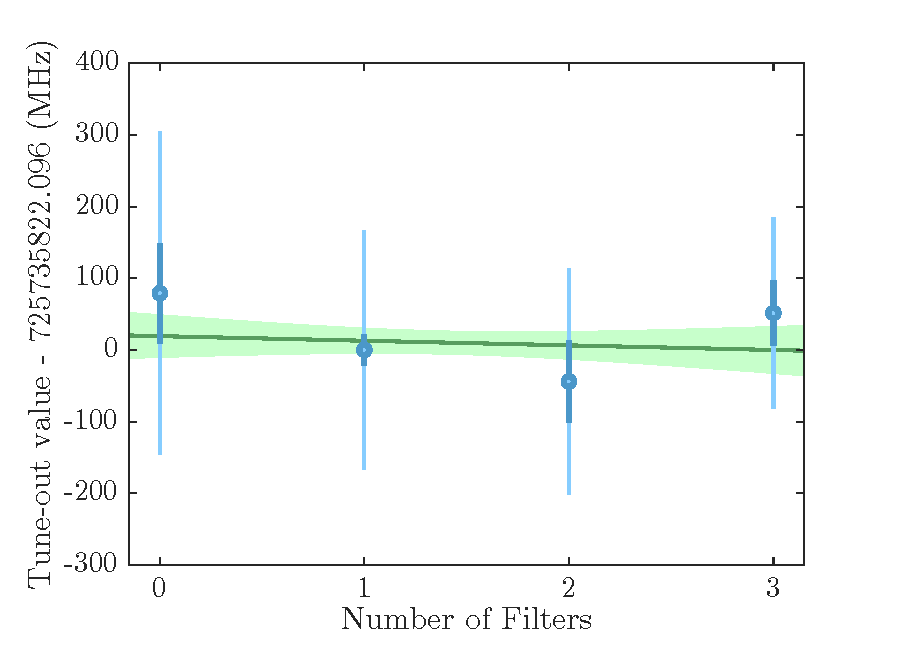
\includegraphics[width=8.6cm]{figs/filt_dep.eps}
\caption{ The dependence of our measurement on increasingly stringent filtering of the laser. The filters are in order [check all these] 450 bluepass, $450\pm15$~nm bandpass, $413pm0.5$~nm
}
\end{figure}






% \begin{figure}[H]
% \centering
% 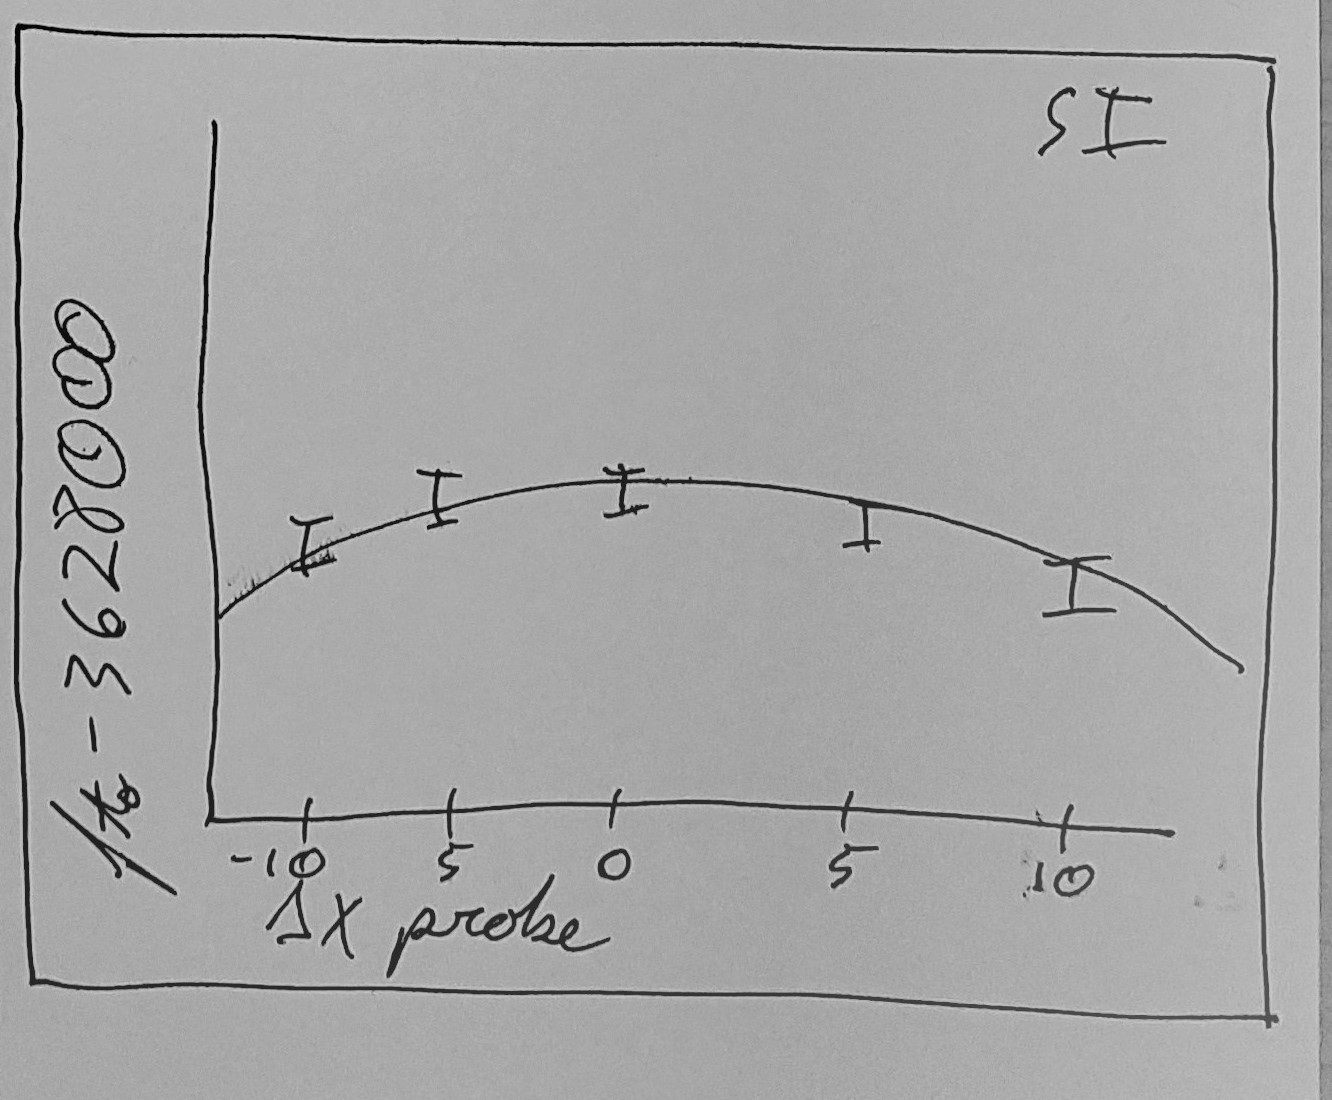
\includegraphics[width=8.6cm]{fig5.jpg}
% \caption{ Measured alingment sensitivity.
% }
% \label{fig:to_align}
% \end{figure}





\end{document}
%
% ****** End of file apssamp.tex ******
